\chapter{Evaluation}

In previous chapters, we've made fairly extensive reasoning behind each part of the algorithm. However, we have yet to see how the algorithm will perform as a whole. In this chapter, the algorithm is tested in various situations.

\section{Case Study}

First part of the evaluation consists of putting the algorithm up against handcrafted sets of obstacles. We can view how particular edge cases are handled, how natural the overall motion is, and if there are any situations it cannot reasonably deal with.

We can now demostrate initial results within a RoFI simulator. As a baseline, we consider a manipulator that consists of a chain of 4 modules, linked via the $-Z$ connectors. Since such a manipulator has 12 degrees of freedom, previous state of the art algorithms -- which mostly only scale up to 6 DoF -- would clearly not be useful.
The simulator does not consider the forces of gravity, or physical failure of the modules; these are aspects of further research. The reasoning behind using 4 modules as the baseline is that such a manipulator is flexible enough even though the joints are constrained, and with the state of the art hardware, it's feasible for the joint of a single module to lift the weight of around 3 connected modules, but not significantly more.

The measurements take place on consumer grade hardware, equipped with 16 GB RAM and an Intel Core i7-8750H cpu.

To evaluate the quality of the algorithm, we want to explore how differently shaped environments affect the algorithm's runtime and ability to find successful paths.

As a sanity check, we can start with a simple case of a target near an obstacle, but reachable from the initial position. The environment is a wall made out of 12 small spheres. Figure~\ref{fig:sim3} shows the performed movement.

\begin{figure}
  \centering
  \begin{minipage}{\textwidth}
    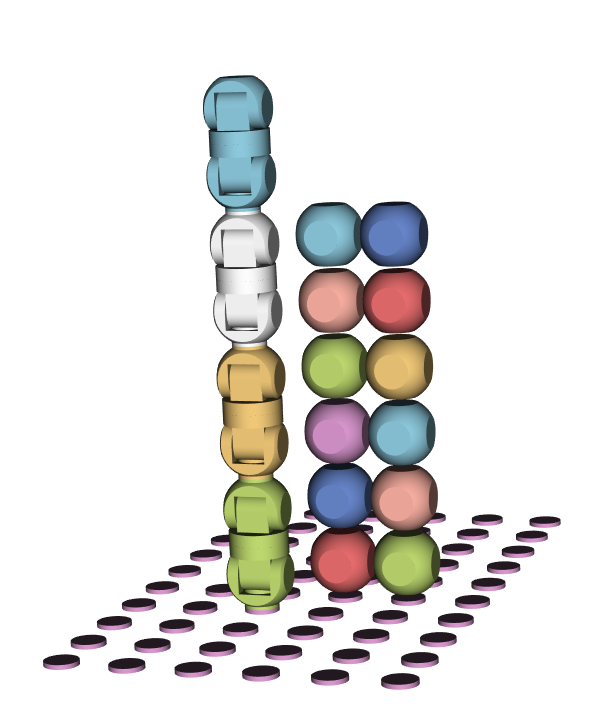
\includegraphics[width=0.24\textwidth]{sim3_0.png}
    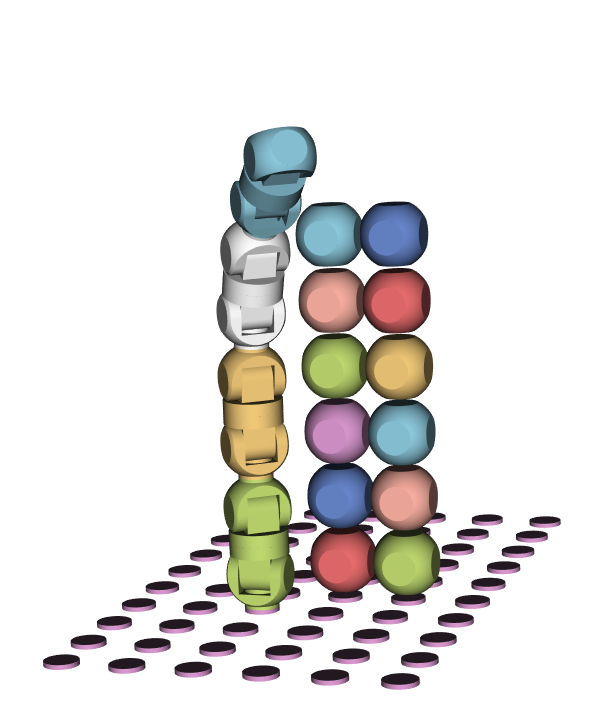
\includegraphics[width=0.24\textwidth]{sim3_1.png}
    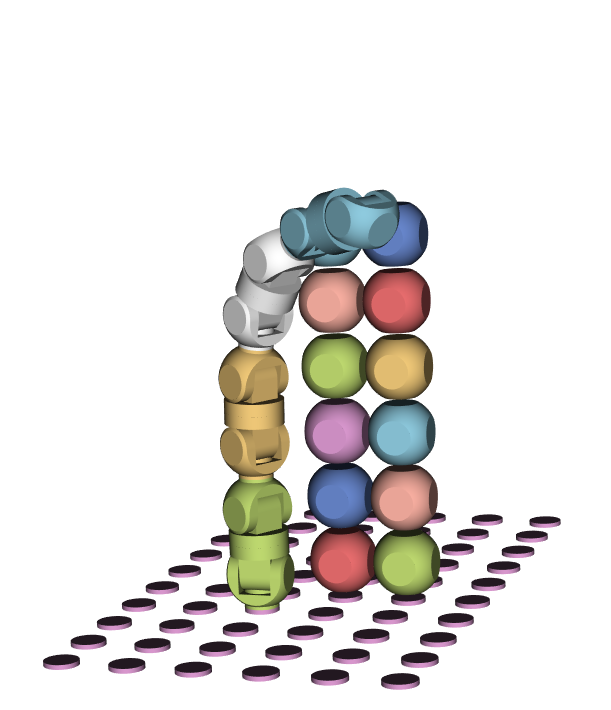
\includegraphics[width=0.24\textwidth]{sim3_2.png}
    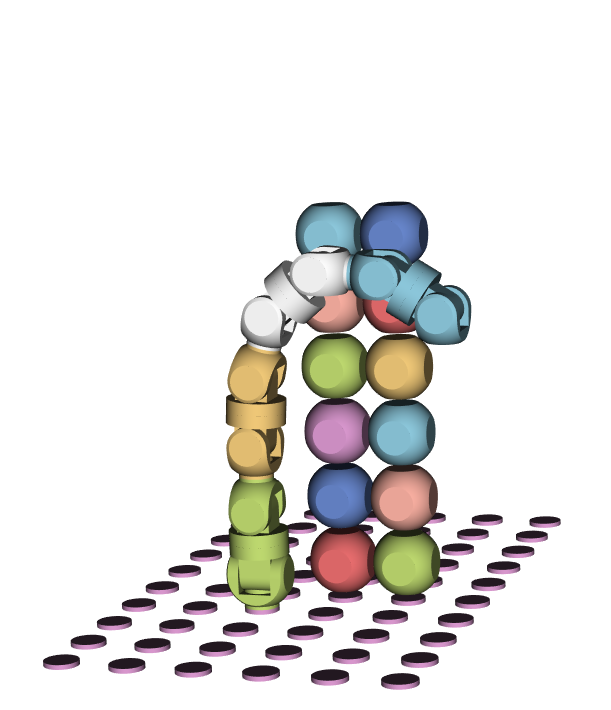
\includegraphics[width=0.24\textwidth]{sim3_3.png}
  \end{minipage}
  \caption{Test case 1: Target near obstacle}\label{fig:sim3}
\end{figure}

A notable feature observable in this case is that even though there is a fairly high number of obstacles, they don't affect the final result in a negative way unless they are in the way. The final position looks very natural, and the performed movement is as smooth as it gets: a direct interpolation between the initial and target position. Since the target is visible from the initial position, the algorithm directly finds the path from it to the target. The whole computation runs for around $0.01$ second.

A more interesting case is observable when we start off in a position close to the wall and try to reach a target behind the wall. In this case, the algorithm needs to first move back to avoid the wall, and then go to the target. The direct path can no longer be taken due to the obstacles, and going around the wall is infeasible due to the limited length of the manipulator. The resulting motion can be seen in Figure~\ref{fig:sim4}.

\begin{figure}[h]
  \centering
  \begin{minipage}{\textwidth}
    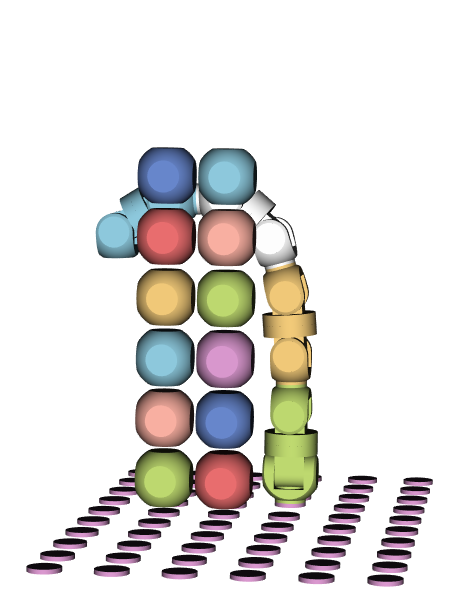
\includegraphics[width=0.24\textwidth]{sim4_0.png}
    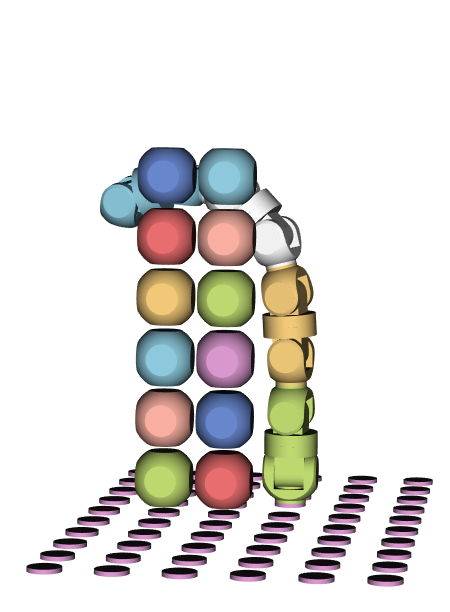
\includegraphics[width=0.24\textwidth]{sim4_1.png}
    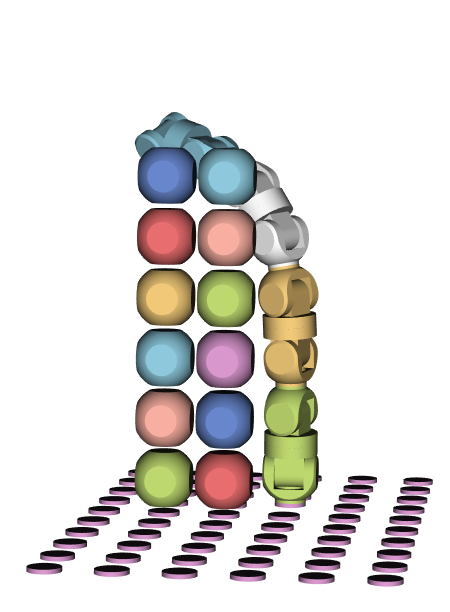
\includegraphics[width=0.24\textwidth]{sim4_2.png}
    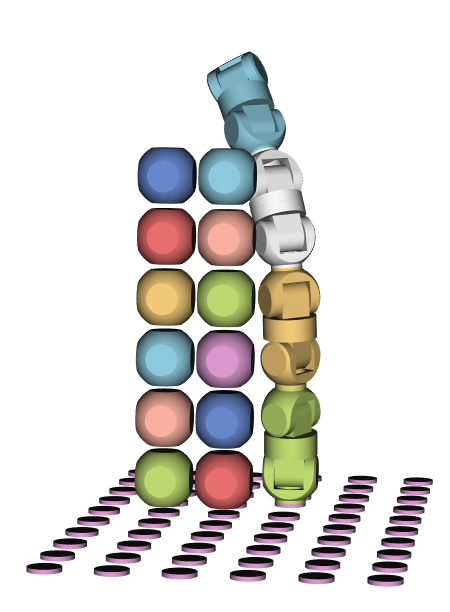
\includegraphics[width=0.24\textwidth]{sim4_3.png}

    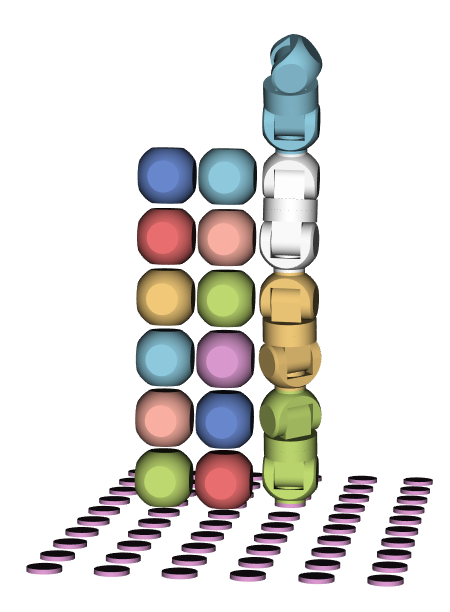
\includegraphics[width=0.24\textwidth]{sim4_4.png}
    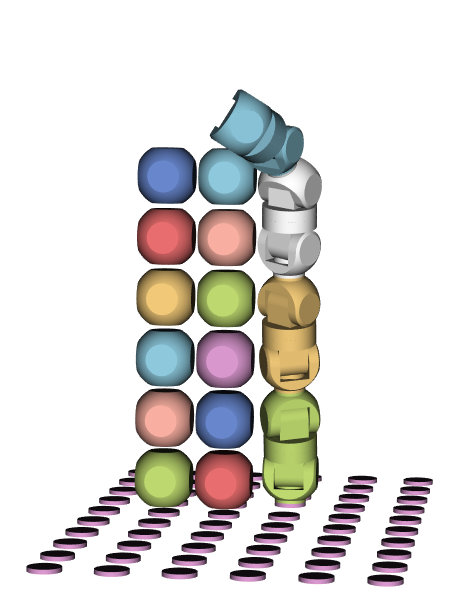
\includegraphics[width=0.24\textwidth]{sim4_5.png}
    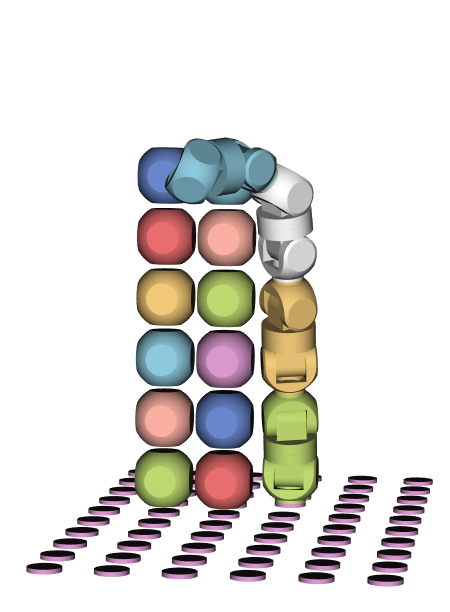
\includegraphics[width=0.24\textwidth]{sim4_6.png}
    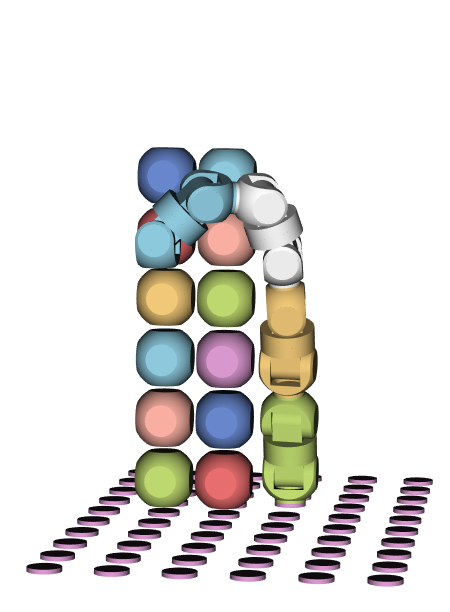
\includegraphics[width=0.24\textwidth]{sim4_7.png}
  \end{minipage}
  \caption{Test case 2: Target behind obstacle}\label{fig:sim4}
\end{figure}

Unlike the first test case, the algorithm doesn't immediately find the right path. Since the paths that lead behind the wall are physically closer, they are evaluated as shorter at first, but trying to folow them fails due to the limited length of the manipulator. On the 5\th{} path, a correct solution that goes around the wall is found. Since we needed to explore multiple paths, each of which is associated with a lot of computation, the solution was found in $0.5$ seconds.

The next test case consists of trying to fit the manipulator in a small hole between obstacles and reach a target behind it. In some cases, this problem has proven to be challenging.
Any path to the target has to go through the hole, but the direction where we come from can play a part as well: in order to fit the joints through the hole, the manipulator needs to move in a fairly specific direction, because there isn't space to move around and readjust when the manipulator goes through the hole. Usually, it does find a solution, see Figure~\ref{fig:sim5}.


\begin{figure}[h]
  \centering
  \begin{minipage}{\textwidth}
    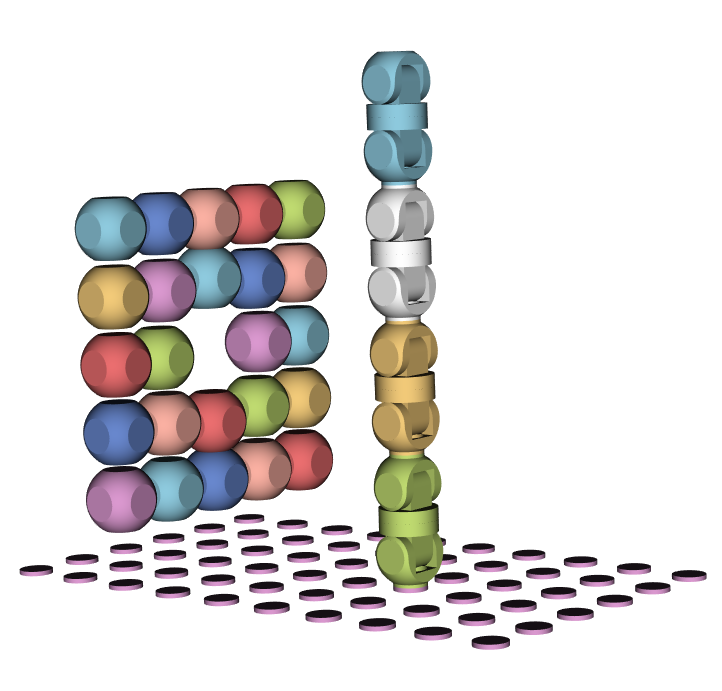
\includegraphics[width=0.24\textwidth]{sim5_0.png}
    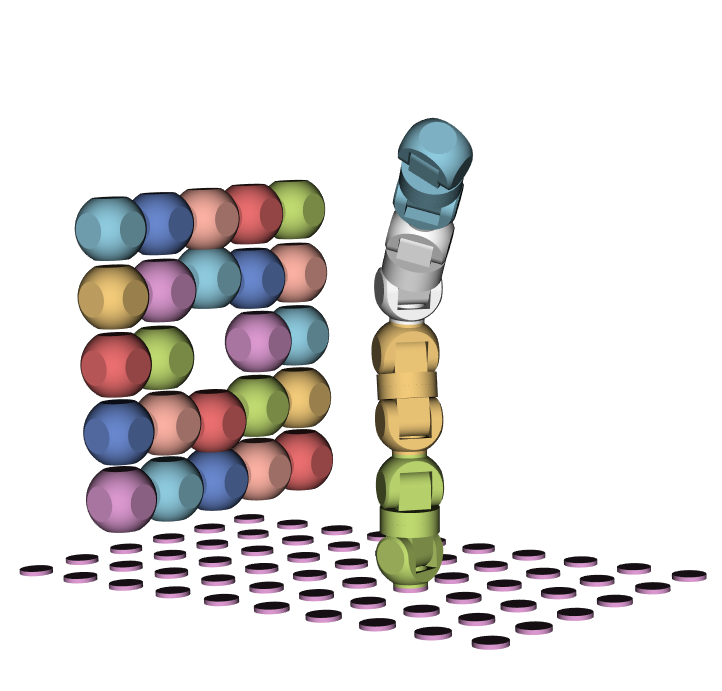
\includegraphics[width=0.24\textwidth]{sim5_1.png}
    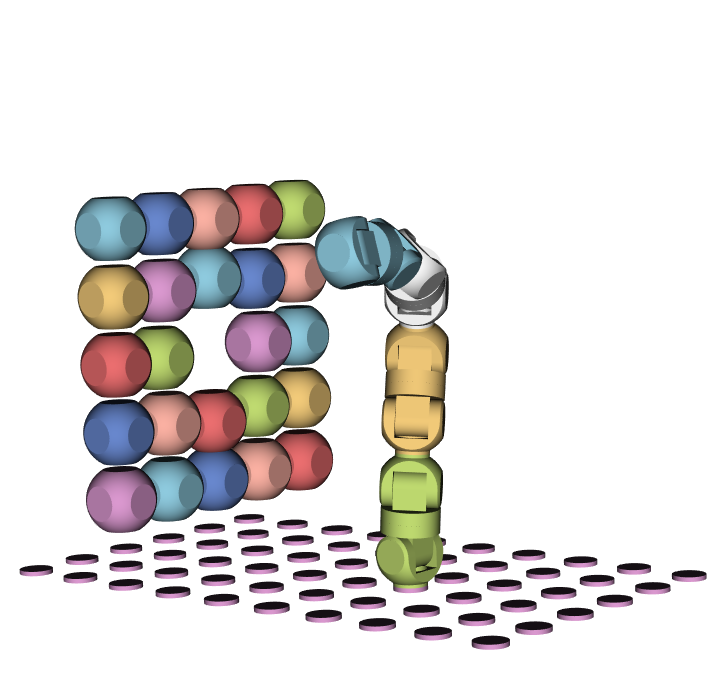
\includegraphics[width=0.24\textwidth]{sim5_2.png}
    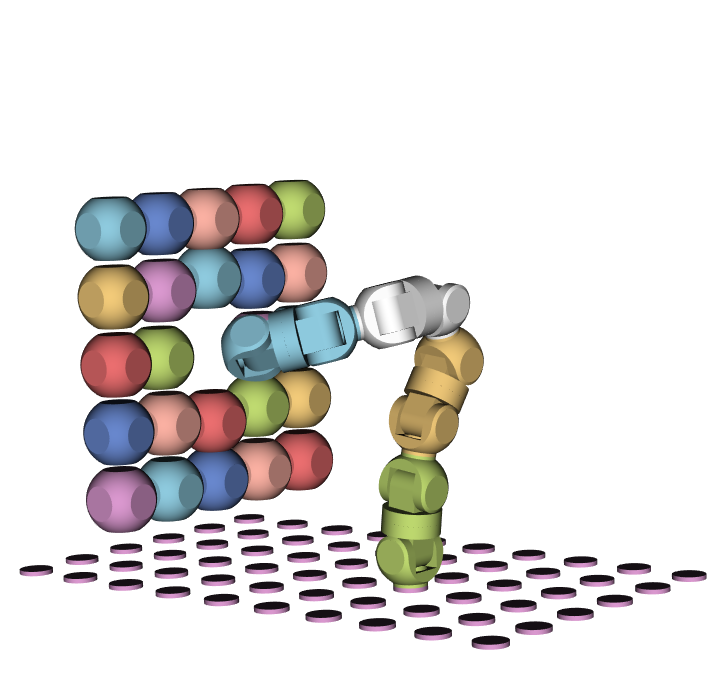
\includegraphics[width=0.24\textwidth]{sim5_3.png}

    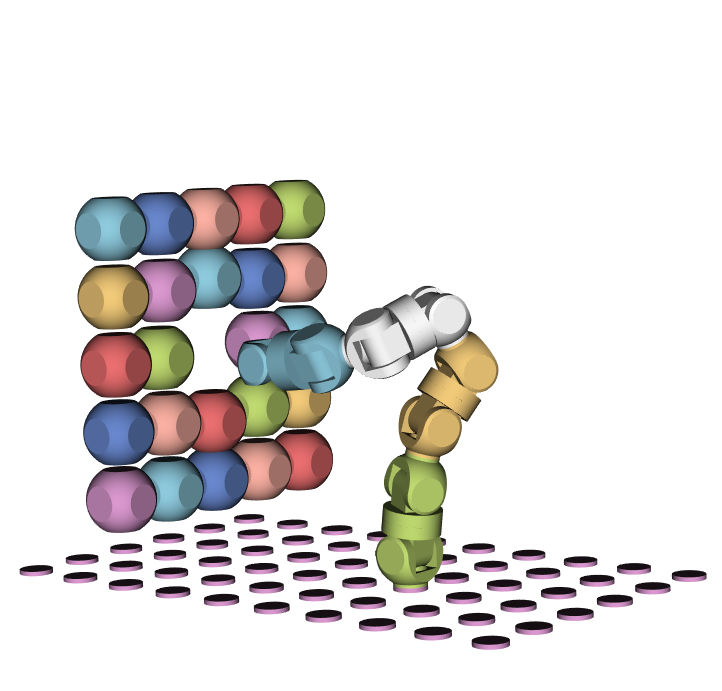
\includegraphics[width=0.24\textwidth]{sim5_4.png}
    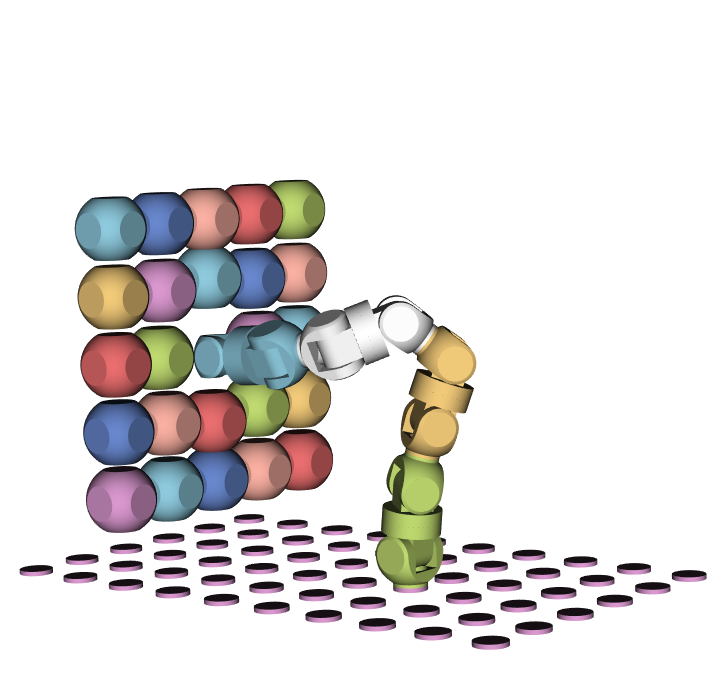
\includegraphics[width=0.24\textwidth]{sim5_5.png}
    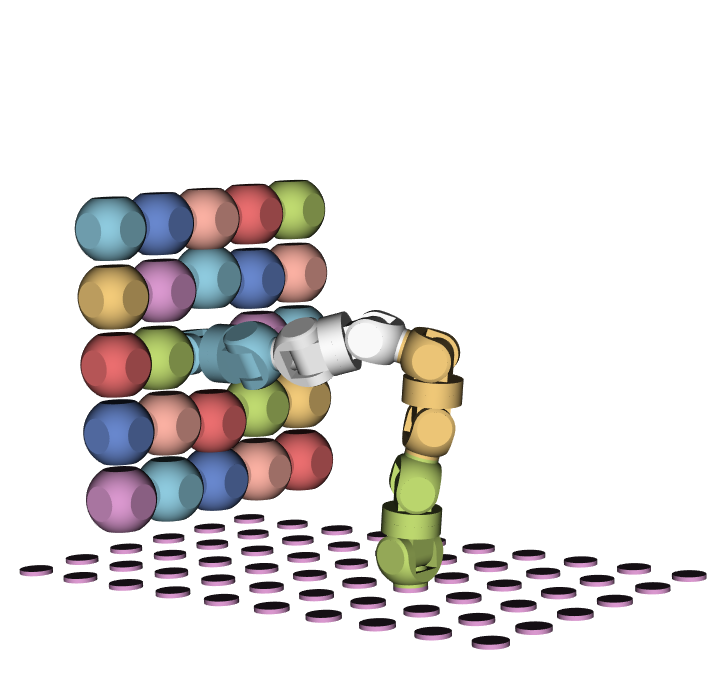
\includegraphics[width=0.24\textwidth]{sim5_6.png}
    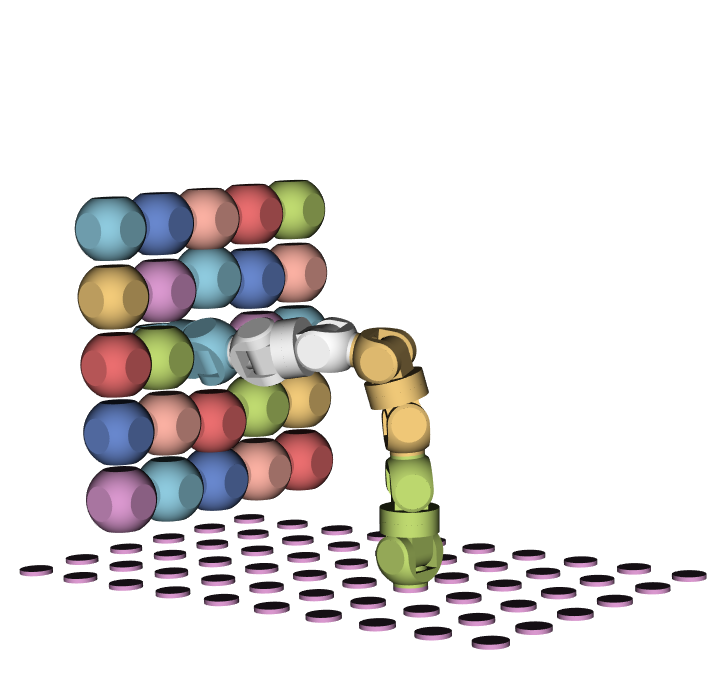
\includegraphics[width=0.24\textwidth]{sim5_7.png}
  \end{minipage}
  \caption{Test case 3: Hole between obstacles}\label{fig:sim5}
\end{figure}

However, if the target is fairly far beyond the hole, but the only way to reach it is to go through it, the algorithm does struggle. Since the point between the obstacles is associated with a high cost, it often tries other paths first, exploring a much larger part of the space compared to the previous examples.

The example~\ref{fig:sim5} was found in $0.04$ seconds, on the first explored path. However, some targets further from the hole can lead to exploring a much larger number of paths; leading to a noticeable delay of a few seconds.

As it stands, the algorithm has its limits. One particular case where it fails to find a viable path in a reasonable time\footnote{The algorithm shuts down after 100 explored paths, which corresponds to up to half a minute of computation time, depending on the complexity of the environment.} is when there is a big wall right in front of the initial \textit{end effector} position, and another one behind it. In our example, see Figure~\ref{fig:d_wall}, we have a floating wall, followed by a small wall, and the target lies beyond both. To reach the goal, the manipulator would have to perform a very complex and specific motion: reach back, curl up under the first wall, go between the walls, and finally reach the goal. Unfortunately, due to how the algorithm works and how constants are set, the manipulator keeps trying to find ways around the walls, with no success. Paths that go down the wall fail due to the fact that there isn't enough space between the manipulator and the wall, and it cannot assume the positions in a natural way.

\begin{figure}
  \centering
  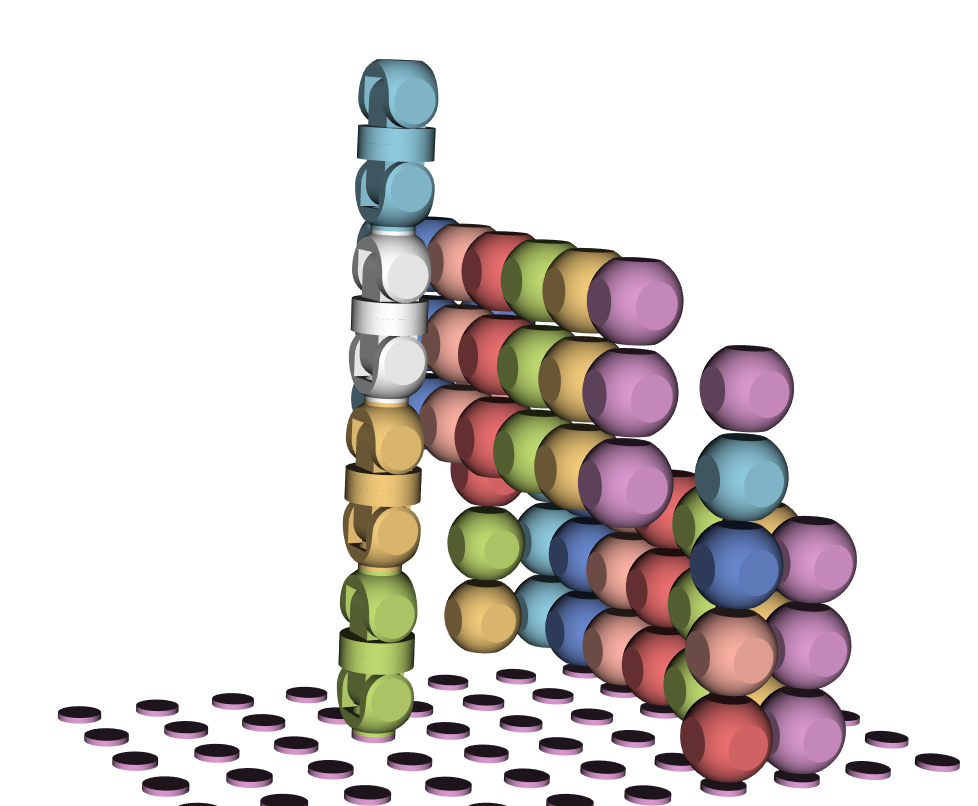
\includegraphics[width=0.8\textwidth]{double_wall.png}
  \caption{Test case 4: Double wall with complex motion}\label{fig:d_wall}
\end{figure}

With minor modifications to the problem, the algorithm does find a viable solution, which gives us some hints for future improvements. The cases where it does find solutions to the problem are:

\begin{itemize}
\item The first wall is a bit further from the manipulator.
\item The walls are not as wide and there is a way around them.
\item The manipulator is not in a straightened out position, but already somewhat curled up at the start of the computation.
\end{itemize}

Moving on, we want to see how the algorithm performs when the obstacles don't form a wall, but instead float in space and form clusters. First up, clusters near the target. This is clearly a practically motivated problem: if we have some objects lying around and need to pick and place a specific one (or a few), we require a precise motion that avoids the other objects.

\begin{figure}[h]
  \centering
  \begin{minipage}{\textwidth}
    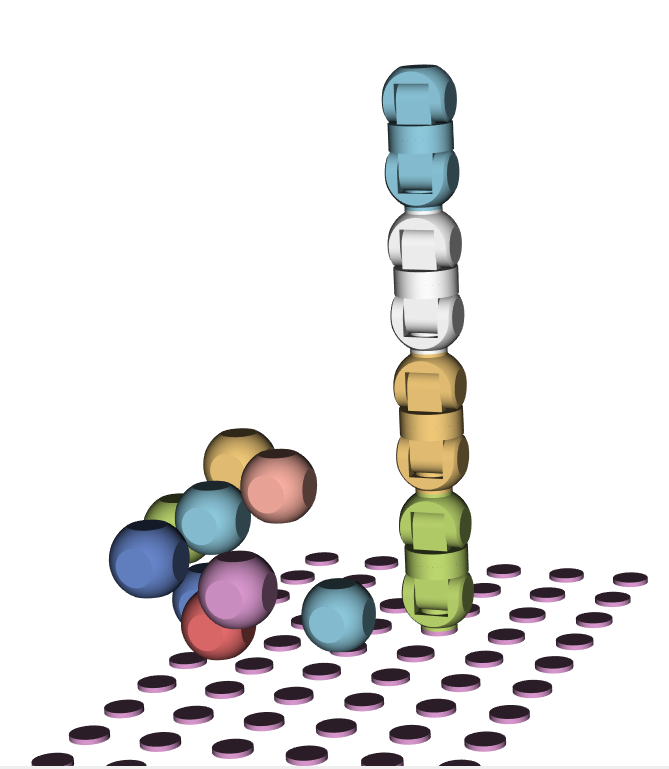
\includegraphics[width=0.3\textwidth]{sim6_0.png}
    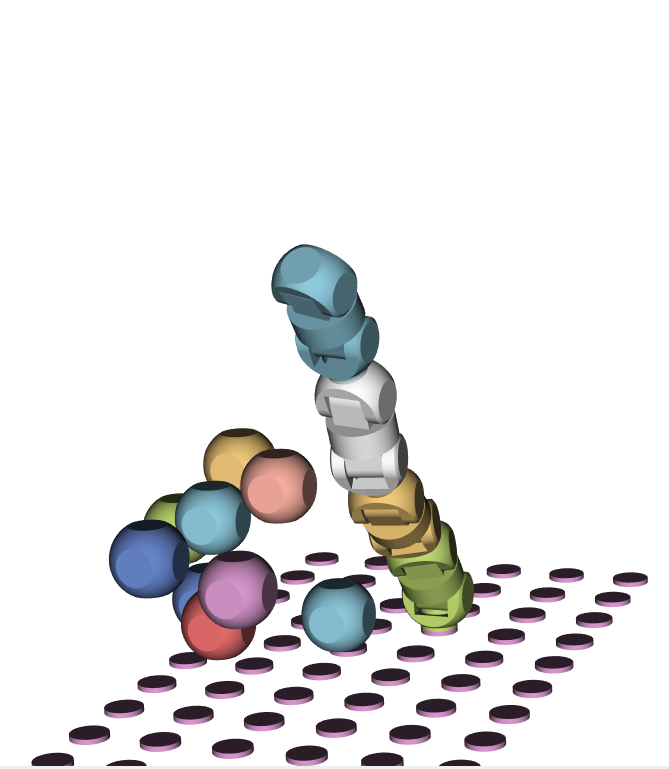
\includegraphics[width=0.3\textwidth]{sim6_1.png}
    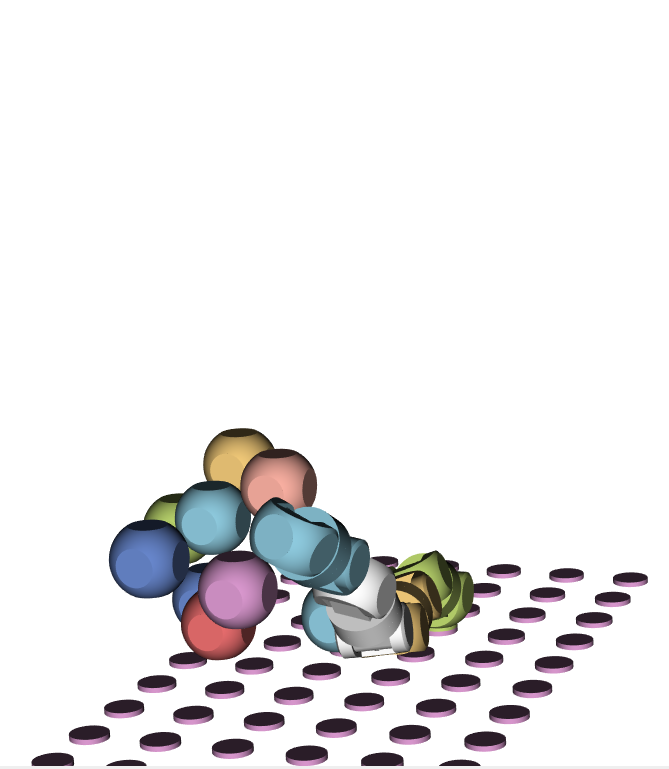
\includegraphics[width=0.3\textwidth]{sim6_2.png}

    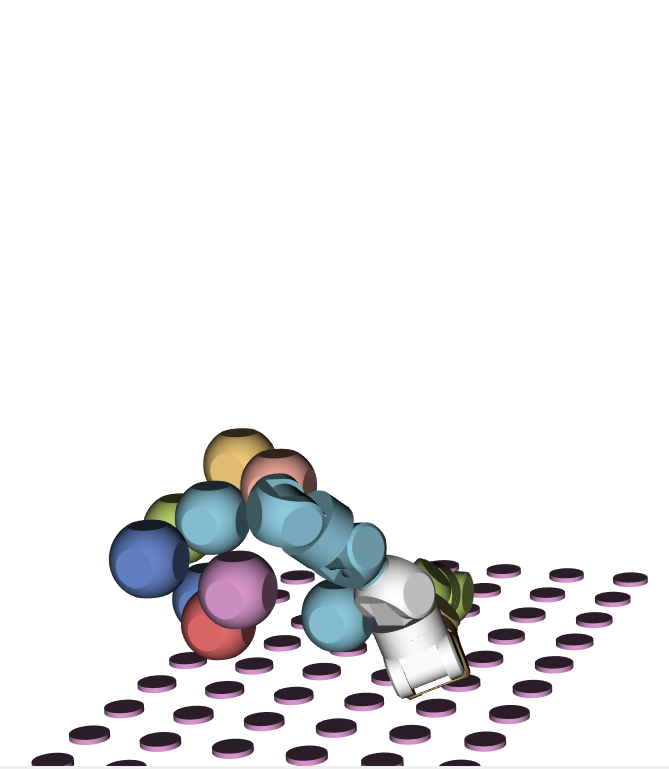
\includegraphics[width=0.3\textwidth]{sim6_3.png}
    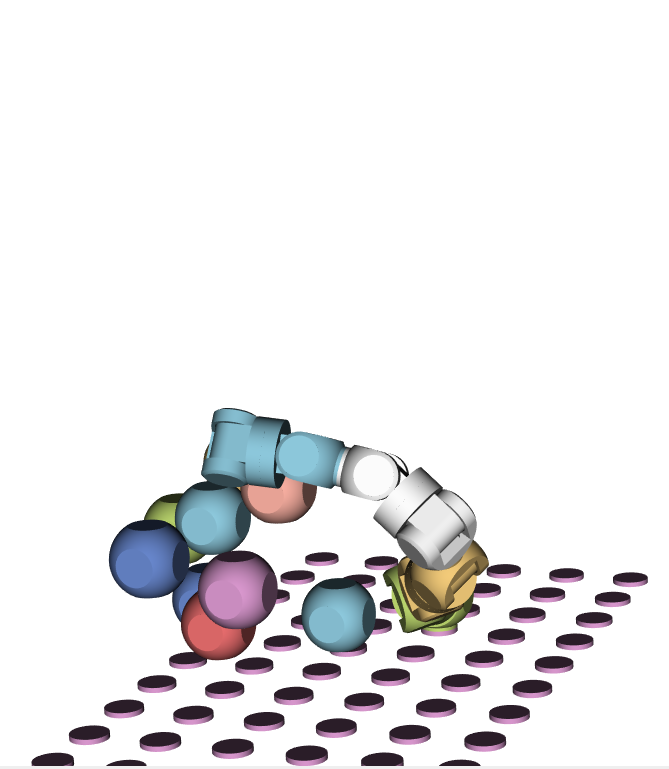
\includegraphics[width=0.3\textwidth]{sim6_4.png}
    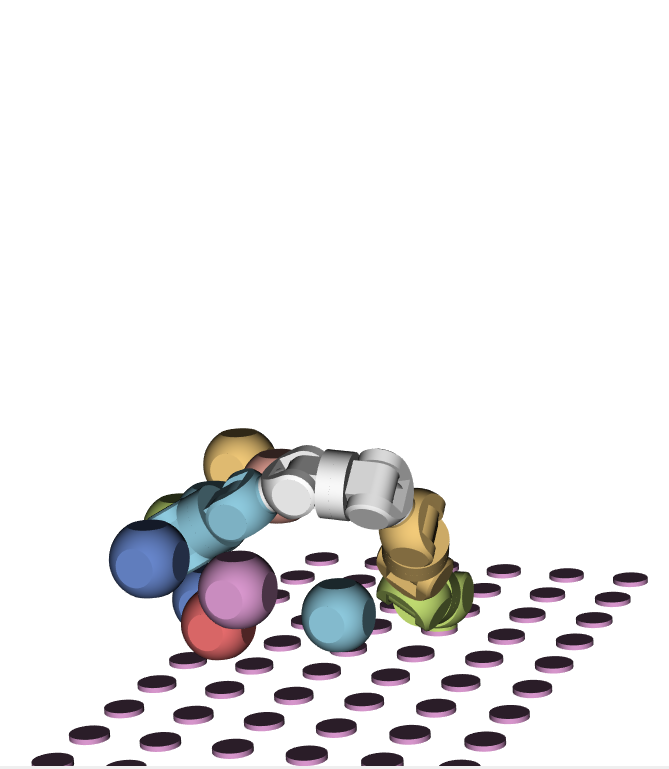
\includegraphics[width=0.3\textwidth]{sim6_5.png}
  \end{minipage}
  \caption{Test case 5: Getting around clusters of objects}\label{fig:sim6}
\end{figure}

The algorithm acts as expected, finding quick and natural looking solutions. Figure~\ref{fig:sim6} shows one example of getting around and between obstacles to reach a target. As designed, the algorithm prioritizes paths that avoid the obstacles altogether and only goes between them at the end of the path if necessary. This often leads to the first evaluated path being correct, which leads to a result in around $0.02$ seconds. When the target lies right in the middle of a cluster and is difficult to navigate into, the algorithm explores multiple paths, but still finishes in less than a second.

Finally, we can take a look at how obstacles affect the manipulator when they aren't close to the manipulator's \textit{end effector}, but rather the lower joints of the manipulator. When the obstacles are all around the manipulator, they don't have as great of an effect on the found paths, compared to when they are surrounding the target. As a result, we need to rely on the quality of our extended FABRIK to avoid them.

\begin{figure}[h]
  \centering
  \begin{minipage}{\textwidth}
    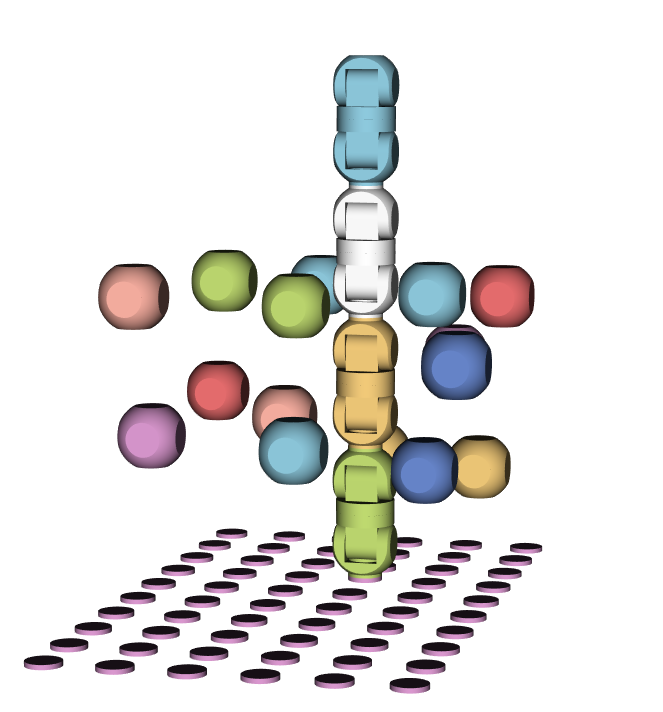
\includegraphics[width=0.24\textwidth]{sim7_0.png}
    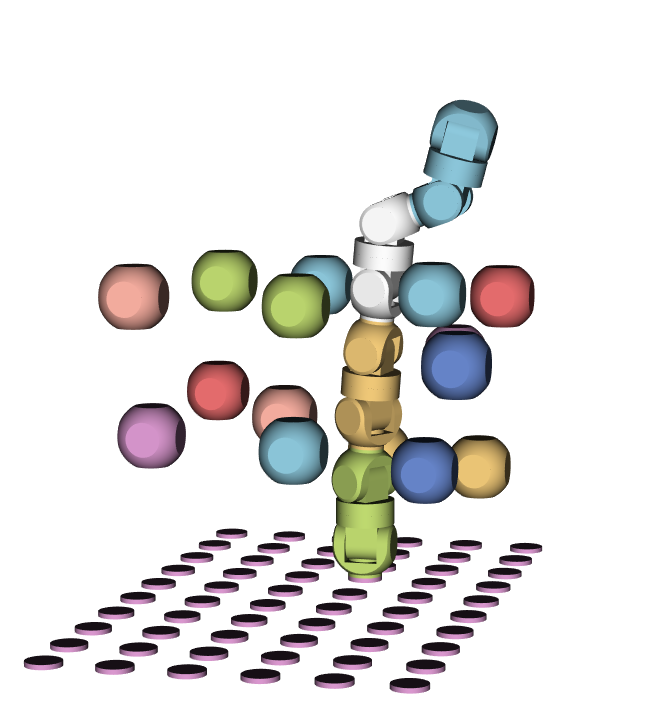
\includegraphics[width=0.24\textwidth]{sim7_1.png}
    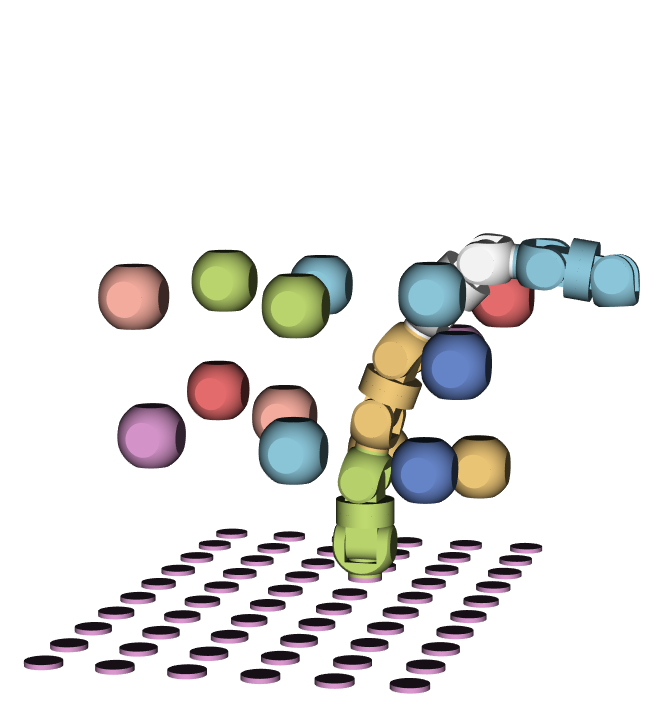
\includegraphics[width=0.24\textwidth]{sim7_2.png}
    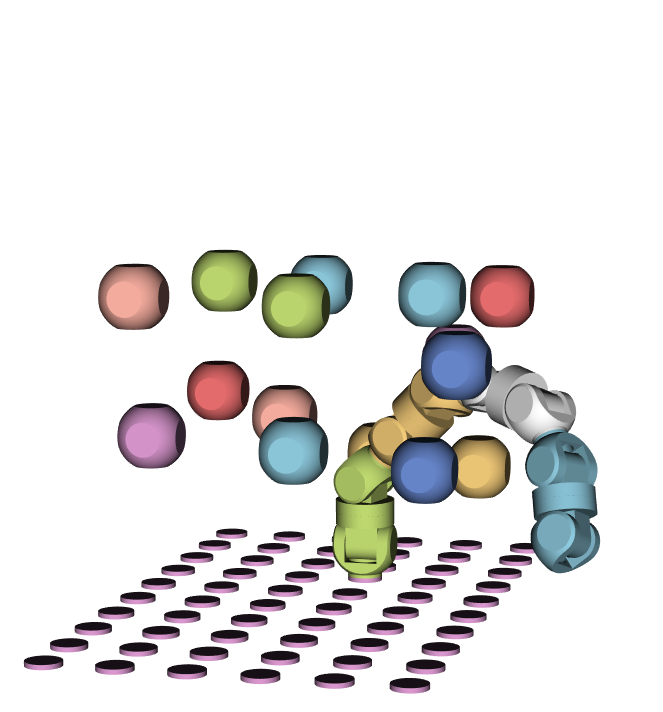
\includegraphics[width=0.24\textwidth]{sim7_3.png}

    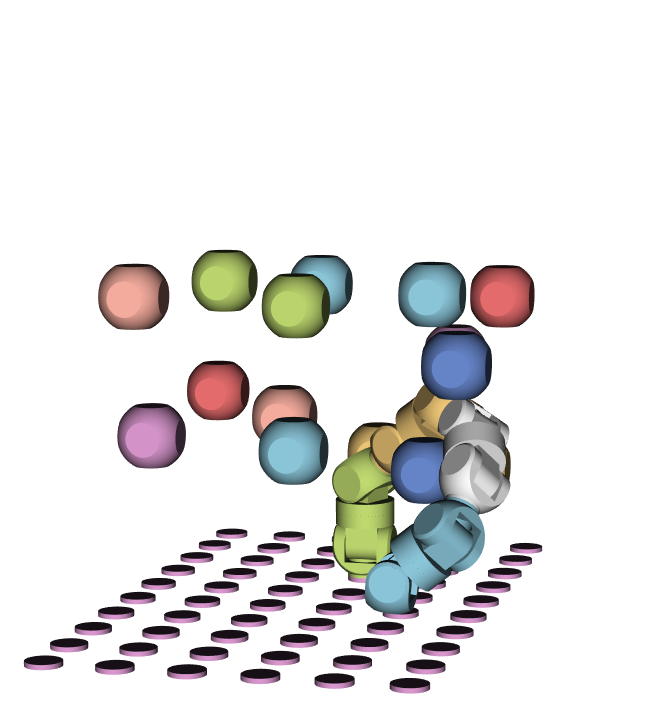
\includegraphics[width=0.24\textwidth]{sim7_4.png}
    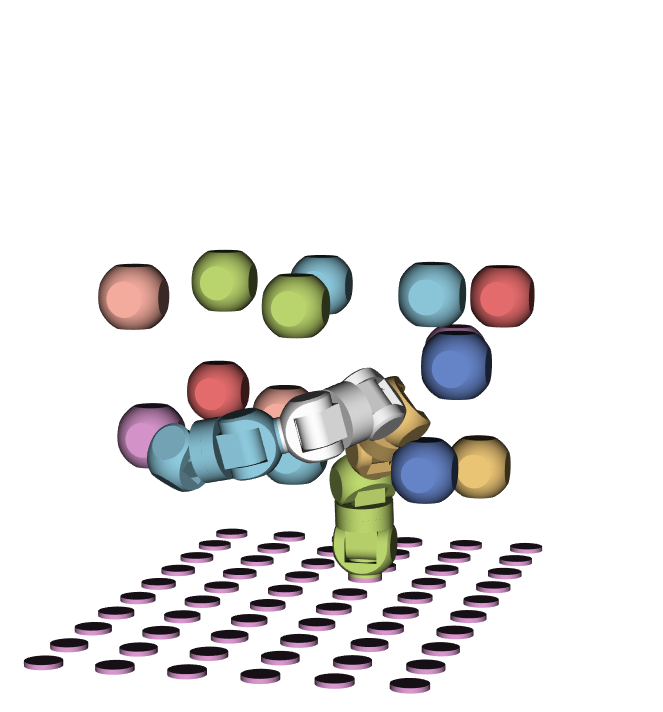
\includegraphics[width=0.24\textwidth]{sim7_5.png}
    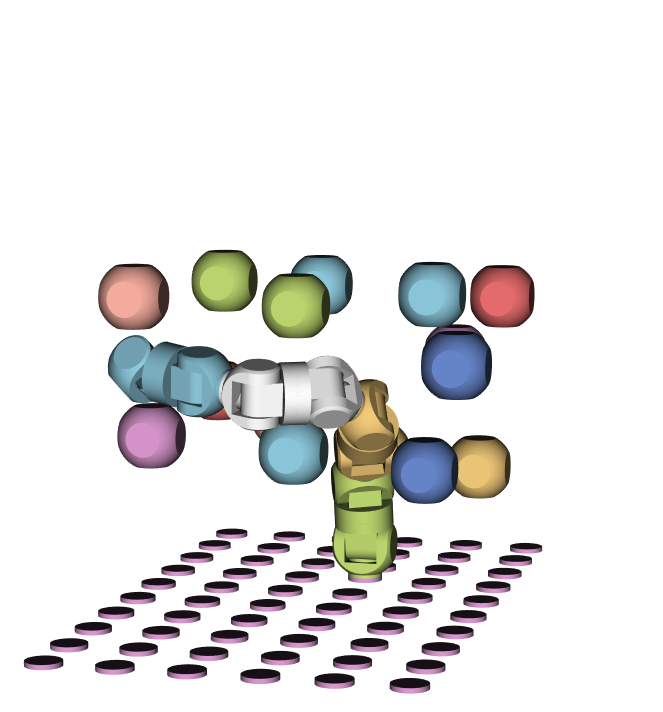
\includegraphics[width=0.24\textwidth]{sim7_6.png}
    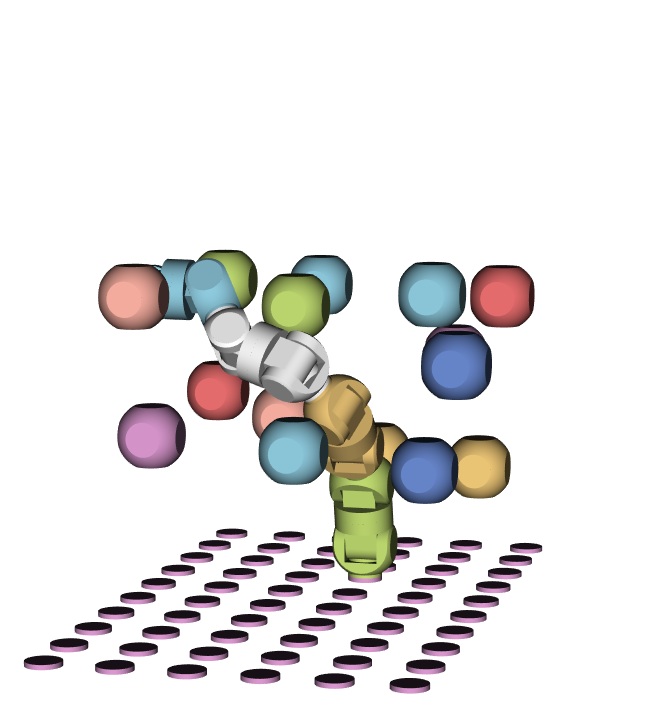
\includegraphics[width=0.24\textwidth]{sim7_7.png}
  \end{minipage}
  \caption{Test case 6: Obstacles all around}\label{fig:sim7}
\end{figure}

The average number of explored paths is higher in this case, and the found paths can stray further from the optimal one. In some cases, the algorithm finds a path close to the expected solution, but since the obstacles in the way have no effect on the resulting path, the manipulator doesn't always find suitable intermediate positions on this path. Even so, the algorithm is capable of navigating through very complex environments, see Figure~\ref{fig:sim7}. We can see that the path of the \textit{end effector} is quite long, and was obviously not the first found solution; it was the 21\st{} path, found after $2$ seconds.

As we can see, the algorithm performs nicely in various environments and finds successful ways to reach the given target. The computation usually runs for less than a second, instantaneous in eyes of a human observer. Reaching some targets takes a couple of seconds, leading to a noticeable delay, but note that the implementation is only a proof of concept, and the given times are referential; there are certainly more optimisations that can be added to the algorithm.

\section{Performance}

Of course, looking at the results on (mostly) handcrafted examples doesn't give us a full picture of the algorithm's overall performance. To evaluate it on a larger scale, we can use an environment with randomly generated obstacles and randomly chosen (reachable) targets. We are interested in how often the algorithm successfully finds a path to the target, how long the individual parts of the computation take, and how well it scales with respect to an increasing number of obstacles and joints.

// TODO: dodělat benchmarking a dát sem tabulky/grafy
